\section{Below 1 Hz}\label{sec:cadence}

\subsection{Why everything is tied to 1 Hz}

Every number of the method counts fixes: the smoothing over 6, the windows over 30, the vote over
90, $\alpha$ in radians per fix, and $A$, which gives the probability of a change between two
consecutive fixes. On a track logged every 5~s the same code would read 30 fixes as two and a half
minutes, compare a 5-s turn with a 1-s threshold, and let phases change five times less often. His
training script keeps only tracks whose mean step is below 1.2~s; the inference script checks
nothing, and would label such a track with the numbers of 1~Hz.

There are two ways around it. One is to rescale every number to the logging interval $\Delta$:
windows of $30/\Delta$ fixes, a new $\alpha$, the matrix $A^\Delta$, a vote over $90/\Delta$ fixes.
Each of these is a new assumption to check, and at 5~s a window of six fixes leaves little to
count. The other is to bring the track to the method: interpolate it onto a regular 1-s grid and
run the method unchanged, keeping the labels of the real fixes only. We take the second, as agreed
on 20 October 2026; what remains to choose is the interpolation.

\subsection{What interpolation does to the features}

Linear interpolation joins two kept fixes with a straight segment. Between them the heading is
constant, and the whole turn of $\Delta$ seconds happens at the kept fix. After the smoothing of
Section~\ref{sec:frame} and the six-fix mean, the average turn per fix comes out right, but its
profile is spiky: a single kept fix weighs on three or four consecutive values
(Figure~\ref{fig:interpolation}). A cubic spline~\cite{deboor2001} bends between the kept fixes
and spreads the turn as the 1-Hz track does. Tremblay et al.~\cite{tremblay2006} compared the
two kinds on tracks of seabirds and seals thinned from a fine resolution: the error on the
positions hardly depended on the method, while the curvilinear ones (Bézier, Hermite, cubic
spline) gave better track lengths than straight segments. Section~\ref{sec:measurement} repeats
their design, with the labels as the quantity compared.

\begin{figure}
\centering
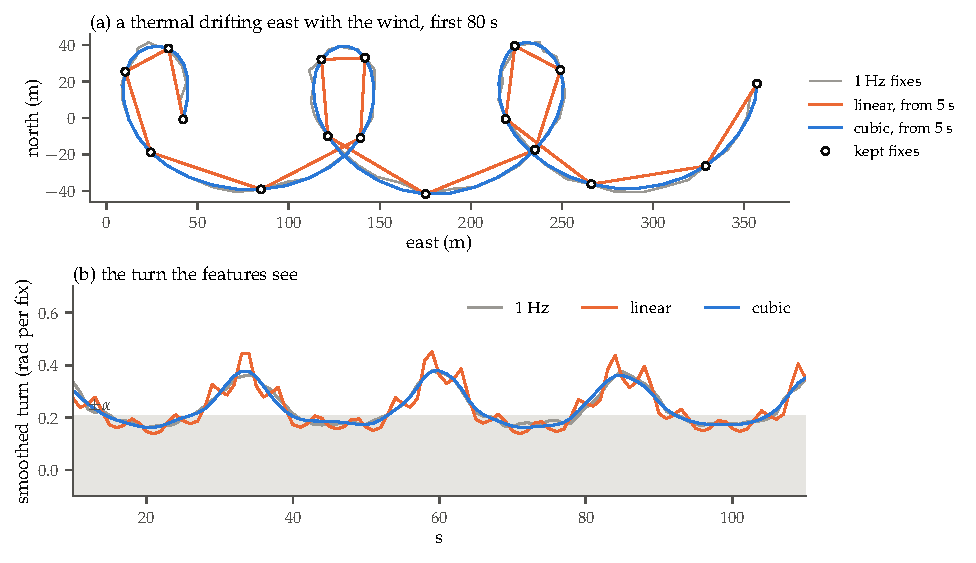
\includegraphics[width=\textwidth]{figures/interpolation.pdf}
\caption{A synthetic thermal, circles of 40~m radius every 26~s drifting east at 4~m/s, climbing at
2~m/s, with 1~m of noise on each 1-Hz fix. (a) The kept fixes, one every 5~s, joined by straight
segments and by a cubic spline. (b) The smoothed turn computed on the 1-Hz track and on the two
interpolations: the linear one is spiky around each kept fix.}
\label{fig:interpolation}
\end{figure}

Two limits follow.
\begin{itemize}
  \item \emph{Aliasing.} The change of heading between two kept fixes is known only modulo $2\pi$,
        so a change larger than $\pi$ reads as a turn the other way. On climbs logged every 5~s
        the median change between kept fixes is 1.26~rad (72\textdegree), 15\% of the changes exceed
        2~rad and 5\% exceed 2.5~rad: drifting circles and tight turns come close to $\pi$. At
        10~s the median is 2.10~rad and a third of the changes exceed 2.5~rad. In possum tracks
        thinned from 5 to 60 minutes the turning angles likewise spread towards a uniform law,
        and a two-state switching walk told the states apart less and less
        clearly~\cite{postlethwaite2013}.
  \item \emph{The one-sign feature.} Rule~\eqref{eq:O} tolerates one disagreement among the 15
        strongest turns of a window. With linear interpolation a kept fix with the wrong sign,
        from GNSS noise or from a change near $\pi$, becomes three or four strong values of the
        wrong sign and switches the feature off. The spline dilutes it.
\end{itemize}

\subsection{The measurement}\label{sec:measurement}

\paragraph{Design.} 300 paraglider flights drawn at random (seed 2026) among those logged every
second that pass the pre-processing and have at least 3600 fixes. In each piece, for
$\Delta=2,3,4,5,10$~s, we keep the fixes whose time is a multiple of $\Delta$, interpolate them onto
a 1-s grid, label, and compare the labels of the kept fixes with the labels the method gives to the
same fixes on the full 1-s piece (\texttt{cadence.py}). The reference is the method at 1~Hz: the
question is whether a coarser logger changes what the method says, and not whether the method is
right.

\paragraph{Results.} Table~\ref{tab:cadence-results} and Figure~\ref{fig:cadence}. Up to 3~s both
interpolations keep about 98--99\% of the labels. From 4~s the linear one loses climbs: at 5~s it
keeps 90.7\% of the climbing fixes and the climb share of the flight drops from 33.3\% to 31.1\%,
while the spline keeps 96.9\% and the share moves by 0.3 points. At 10~s both fail, with fewer than
six climbing fixes in ten kept. Figure~\ref{fig:cadence-example} shows the 5-s case on one flight.

\begin{table}
\centering
\small
\setlength{\tabcolsep}{5pt}
\begin{tabular}{@{}r l r r r r r r@{}}
\toprule
$\Delta$ & interp. & fixes & same label & climb kept & search kept & climb share & worst 10\% \\
\midrule
2~s & linear & 1\,683\,979 & 98.9\% & 99.0\% & 95.8\% & 33.3\% & 97.0\% \\
    & cubic  &             & 99.0\% & 99.0\% & 97.2\% & 33.3\% & 97.2\% \\ \addlinespace
3~s & linear & 1\,125\,818 & 98.2\% & 98.2\% & 92.7\% & 33.2\% & 95.6\% \\
    & cubic  &             & 98.8\% & 98.8\% & 96.1\% & 33.3\% & 96.4\% \\ \addlinespace
4~s & linear & 844\,257 & 97.1\% & 96.4\% & 89.4\% & 32.8\% & 94.1\% \\
    & cubic  &          & 98.3\% & 98.3\% & 94.1\% & 33.3\% & 96.1\% \\ \addlinespace
5~s & linear & 676\,249 & 94.8\% & 90.7\% & 86.2\% & 31.1\% & 89.3\% \\
    & cubic  &          & 97.5\% & 96.9\% & 91.3\% & 33.0\% & 94.7\% \\ \addlinespace
10~s & linear & 338\,359 & 73.2\% & 33.1\% & 81.7\% & 12.6\% & 58.7\% \\
     & cubic  &          & 81.4\% & 57.0\% & 71.6\% & 20.8\% & 69.6\% \\
\bottomrule
\end{tabular}
\caption{Labels of thinned flights against the labels of the full 1-s flights, on the kept fixes.
``Climb kept'' is the share of the fixes labelled climb at 1~Hz that are still climb; the climb
share is 33.3\% at 1~Hz; ``worst 10\%'' is the agreement that 10\% of the flights fall below.}
\label{tab:cadence-results}
\end{table}

\begin{figure}
\centering
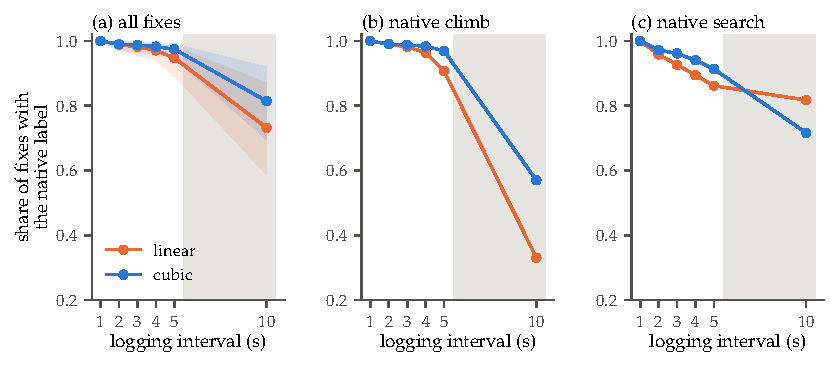
\includegraphics[width=\textwidth]{figures/cadence.pdf}
\caption{Share of the kept fixes that keep their 1-Hz label, against the logging interval: (a) all
fixes, with the band between the 10\% and 90\% of the flights; (b) fixes labelled climb at 1~Hz;
(c) fixes labelled search at 1~Hz. Grey: beyond 5~s.}
\label{fig:cadence}
\end{figure}

\begin{figure}
\centering
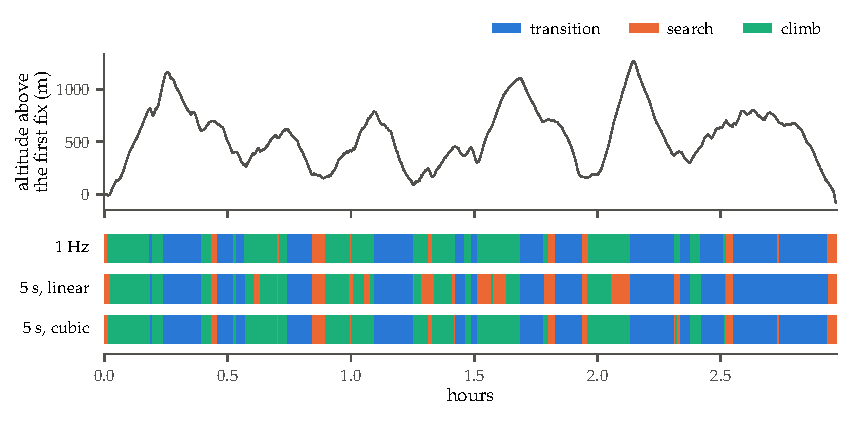
\includegraphics[width=\textwidth]{figures/cadence_example.pdf}
\caption{The flight of Figure~\ref{fig:flight}, labelled at 1~Hz and from one fix every 5~s. With
linear interpolation several climbs turn into searches; with the spline they come back. This flight
is in the worst tenth of the sample for the linear case: it keeps 87\% of its labels against 98.5\%
with the spline.}
\label{fig:cadence-example}
\end{figure}

\paragraph{Mechanism.} On 40 of the flights (\texttt{mechanism.py}), 5.6\% of the climbing fixes
change their symbol from $(0,1,1)$ to $(0,1,0)$ at 5~s with linear interpolation, against 1.2\%
with the spline: the one-sign feature is the one that fails. The share of climbing windows with at
least two strong turns of the minority sign grows from 8.4\% at 1~Hz to 12.9\% with linear
interpolation, and stays at 8.9\% with the spline.

\subsection{Verdict}

\begin{keypoint}{Up to one fix every 5 seconds: yes, with a cubic spline.}
Interpolating each piece onto a 1-s grid with a cubic spline and running the method unchanged
reproduces the 1-Hz labels on 99.0\% of the fixes at 2~s and 97.5\% at 5~s, and keeps the share of
each phase within half a point. Linear interpolation is enough up to 3~s and loses climbs from 4~s
on. At 10~s neither works, because the turns between two fixes reach $\pi$. Flights logged every
more than 5~s stay unlabelled: those at 10~s alone are 2.4\% of the paragliders and 15.2\% of the
hang gliders (Table~\ref{tab:cadence}).
\end{keypoint}

One caveat. Thinning a 1-Hz track keeps its receiver: a logger that records every 5~s may average
or filter its positions, and its errors are those of its own receiver. A visual check on a few
flights logged natively every 5~s, before using them, settles it.
